\section{Civilunrest Forecasting}
The following section gives some case studies of EMBERS forecasts over
the past few years in Latin America.
\subsection{Successful Forecasts}
The following section gives some examples of successful civilunrest
forecasts by the EMBERS system during 2013-2015.

\textbf{Brazil Spring (June 2013)}: These protests were the largest and most
significant protests in Brazil`s recent history that caught worldwide
attention. Millions of Brazilians took part in these demonstrations,
also known as the Brazilian Spring or the Vinegar Movement (inspired
from the use of vinegar soaked cloth by demonstrators to protect
themselves from police teargas), which were catalyzed by an increase in
public transport fares from $R\$3$ to $R\$3.20$ by the government of President
Dilma Rousseff.

As shown in Figure.~\ref{fig:brazilJune13} EMBERS, while missing the initial uptick,
captured the increase in the order of magnitude of the protest events
during the Brazilian Spring and also captured
the spatial spread in the events, in addition to forecasting that this would be
a "General Population" protest.

\begin{figure}[H]
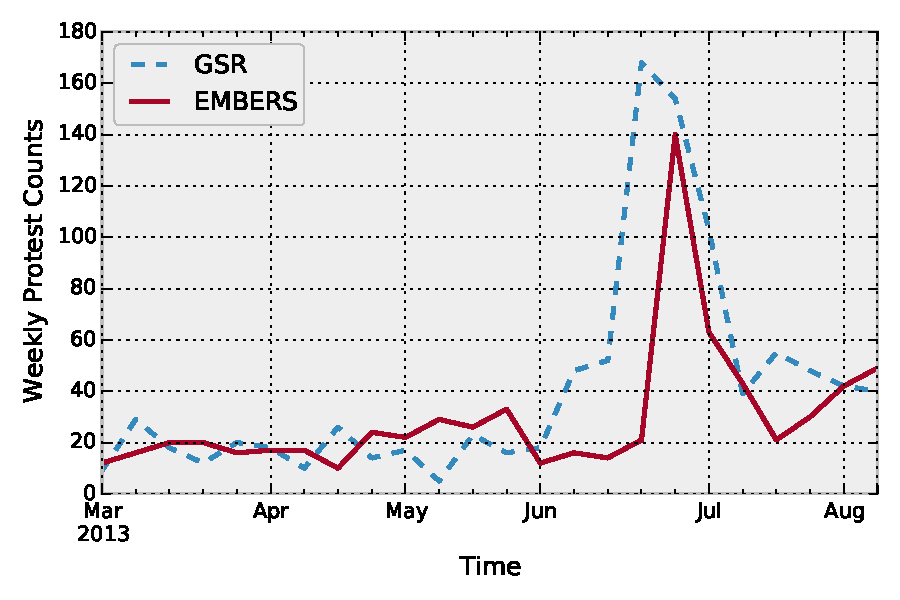
\includegraphics[width=.8\columnwidth]{cu/brazilJune13}
\caption{Brazil Spring}
\label{fig:brazilJune13}
\end{figure}

Around 68\% of EMBERS Brazil alerts resulted from detected planned
protest which can be explained from the fact that the social networking
sites (Twitter and Facebook) and conventional news media played a key
role in organization of these uprisings. Although, initial protests were
mostly against the bus fare increase soon these grew from general
population's deep dissatisfactions to include wider issues such as -
government corruption, over-spending and police brutality. Also,
demonstrators made calls for political reforms. In response, President
Rousseff proposed a referendum on widespread political reforms in
Brazil, but was later abandoned. EMBERS models were able to capture such
discussions on Twitter (see Figure.~\ref{fig:brazilJune13_wordCloud}), and followed these stories as
they evolved through June.

\begin{figure}[H]
\centering
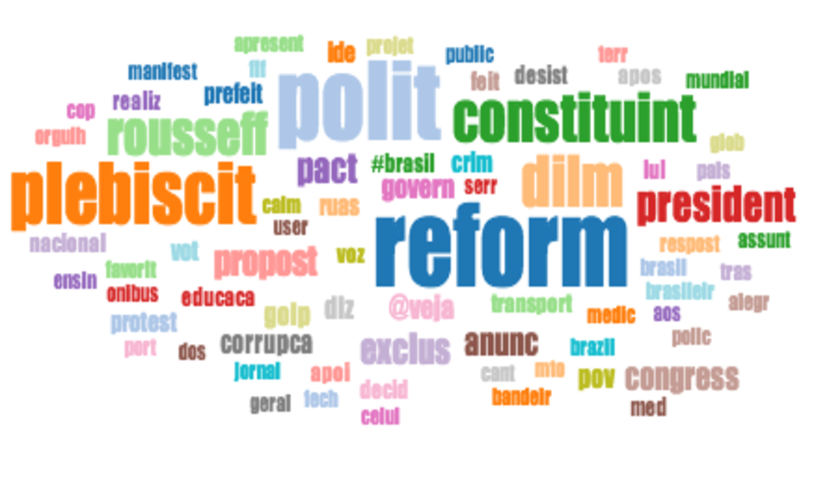
\includegraphics[width=.8\columnwidth]{cu/brazilJune13_wordCloud}
\caption{Word cloud from data extracted by EMBERS models}
\label{fig:brazilJune13_wordCloud}
\end{figure}

The protests intensified in late June (see Figure.~\ref{fig:brazilJune13}), which were
captured by EMBERS, as they also coincided with FIFA 2013 Confederations
Cup matches. This was an important factor due to which protests gained
momentum as they were covered by world media. Majority of protests
occurred in those cities, which were hosting (FIFA) soccer matches.
EMBERS submitted most of its alerts for these host cities (see Figure
~\ref{fig:brazilJune13_map}){\textemdash} Rio de Janeiro, São Paulo,
Belo Horizonte, Salvador and Porto Alegre,
among others. For example, on 27th June during Confederations cup
semi-final in Fortaleza, around 5000 protestors clashed with the police
near the Castelao stadium - In this case EMBERS sent out an alert the
day before. Then later on 30th June, when the last games of the
confederation cup took place in Rio de Janeiro and Salvador that were
also plagued by mass protests – EMBERS predicted these events and
submitted multiple alerts for Rio on 28th and 29th June and one for
Salvador on 29th June.

\begin{figure}[H]
\centering
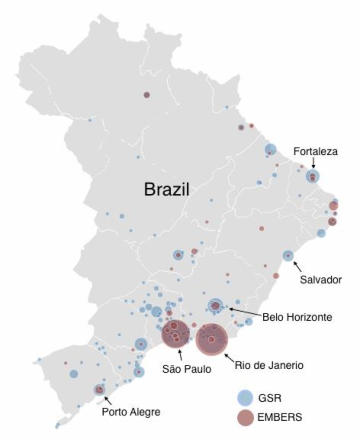
\includegraphics[height=.6\columnwidth]{cu/brazilJune13_map}
\caption{Geographic overlap of Groud Truth protest events and EMBERS
alerts for Brazil June 2013.}
\label{fig:brazilJune13_map}
\end{figure}

\textbf{Venezuelan Spring (Feb-March 2014)}:
EMBERS captured some of the first `calls to protest` for the trigger city of
San Cristobal and its nearby surrounding areas and correctly forecast the
population (Education) and that the protests would turn violent. Over the next
days, EMBERS closely forecast the spike in the number of events as shown
in Figure.~\ref{fig:venezuelaMarch14} and the spread
of the protests to additional cities as shown in
Figure.~\ref{fig:venezuelaMap}.

\begin{figure}[H]
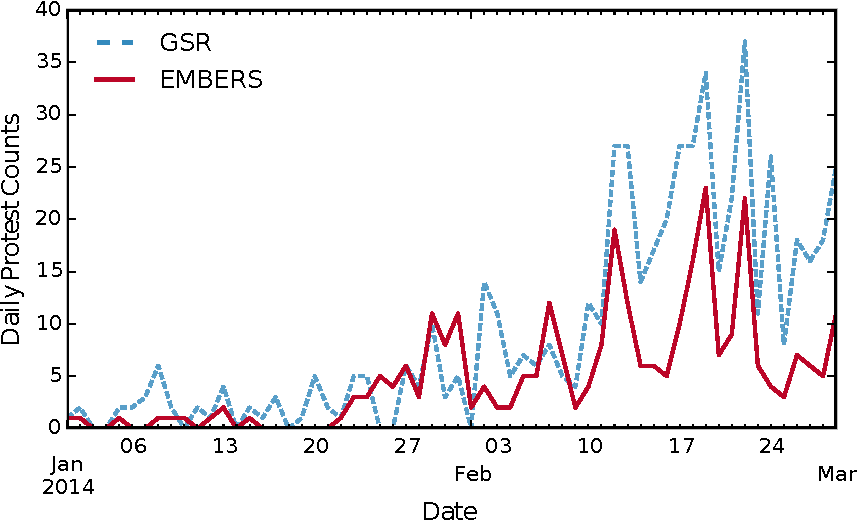
\includegraphics[width=.8\columnwidth]{cu/venezuelaFeb14}
\caption{Venezuelan Spring}
\label{fig:venezuelaMarch14}
\end{figure}

\begin{figure}[H]
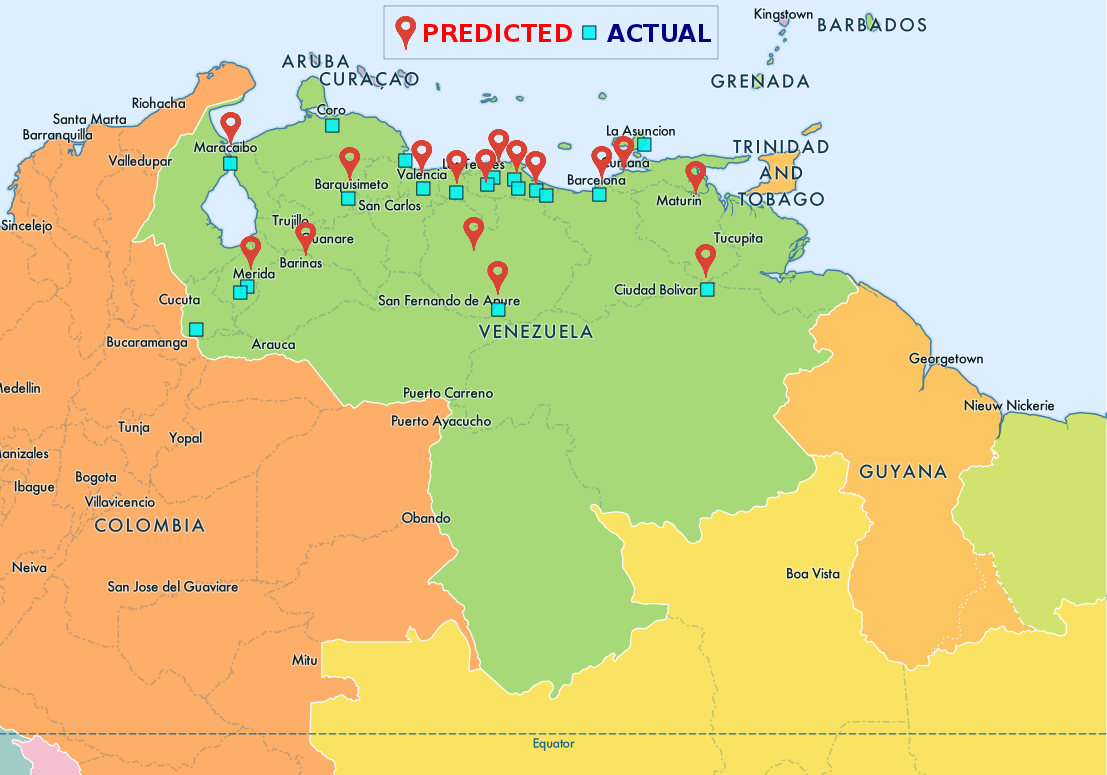
\includegraphics[width=.6\columnwidth]{cu/venezuelaMap}
\caption{Venezuelan Spring}
\label{fig:venezuelaMap}
\end{figure}

\textbf{Mexico Protests (October 2014)}:
EMBERS , as shown in Figure.~\ref{fig:mexicoOct14} forecast an uptick of Mexico
protests during early October 2014 stemming from students and teachers demanding
action on the 43 students missing case, with a lead time of about 3
days. It also generated  a series of alert spikes coinciding with the first
large-scale nationwide protests between October 5th to 8th.

\begin{figure}[H]
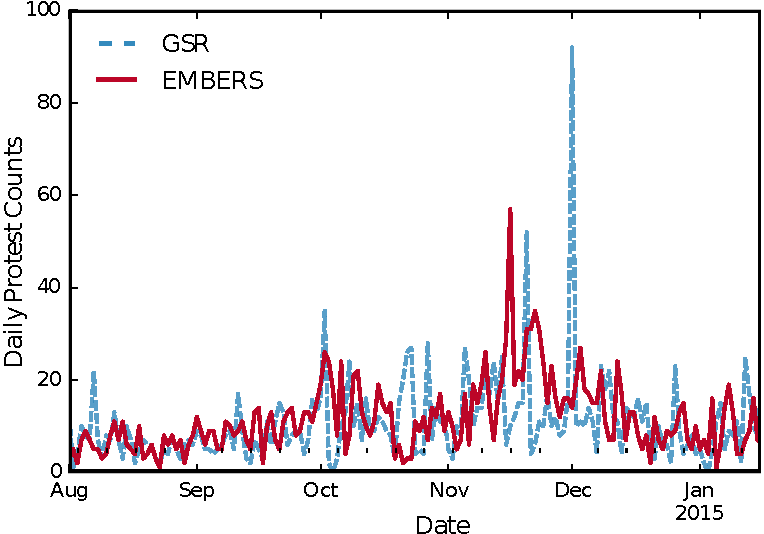
\includegraphics[width=.8\columnwidth]{cu/mexicoOct14}
\caption{Mexico Protests}
\label{fig:mexicoOct14}
\end{figure}

Figure.~\ref{fig:mexicoTimeline} provides a timeline of GSR events and
EMBERS alerts for Mexico during this period
\begin{figure}[H]
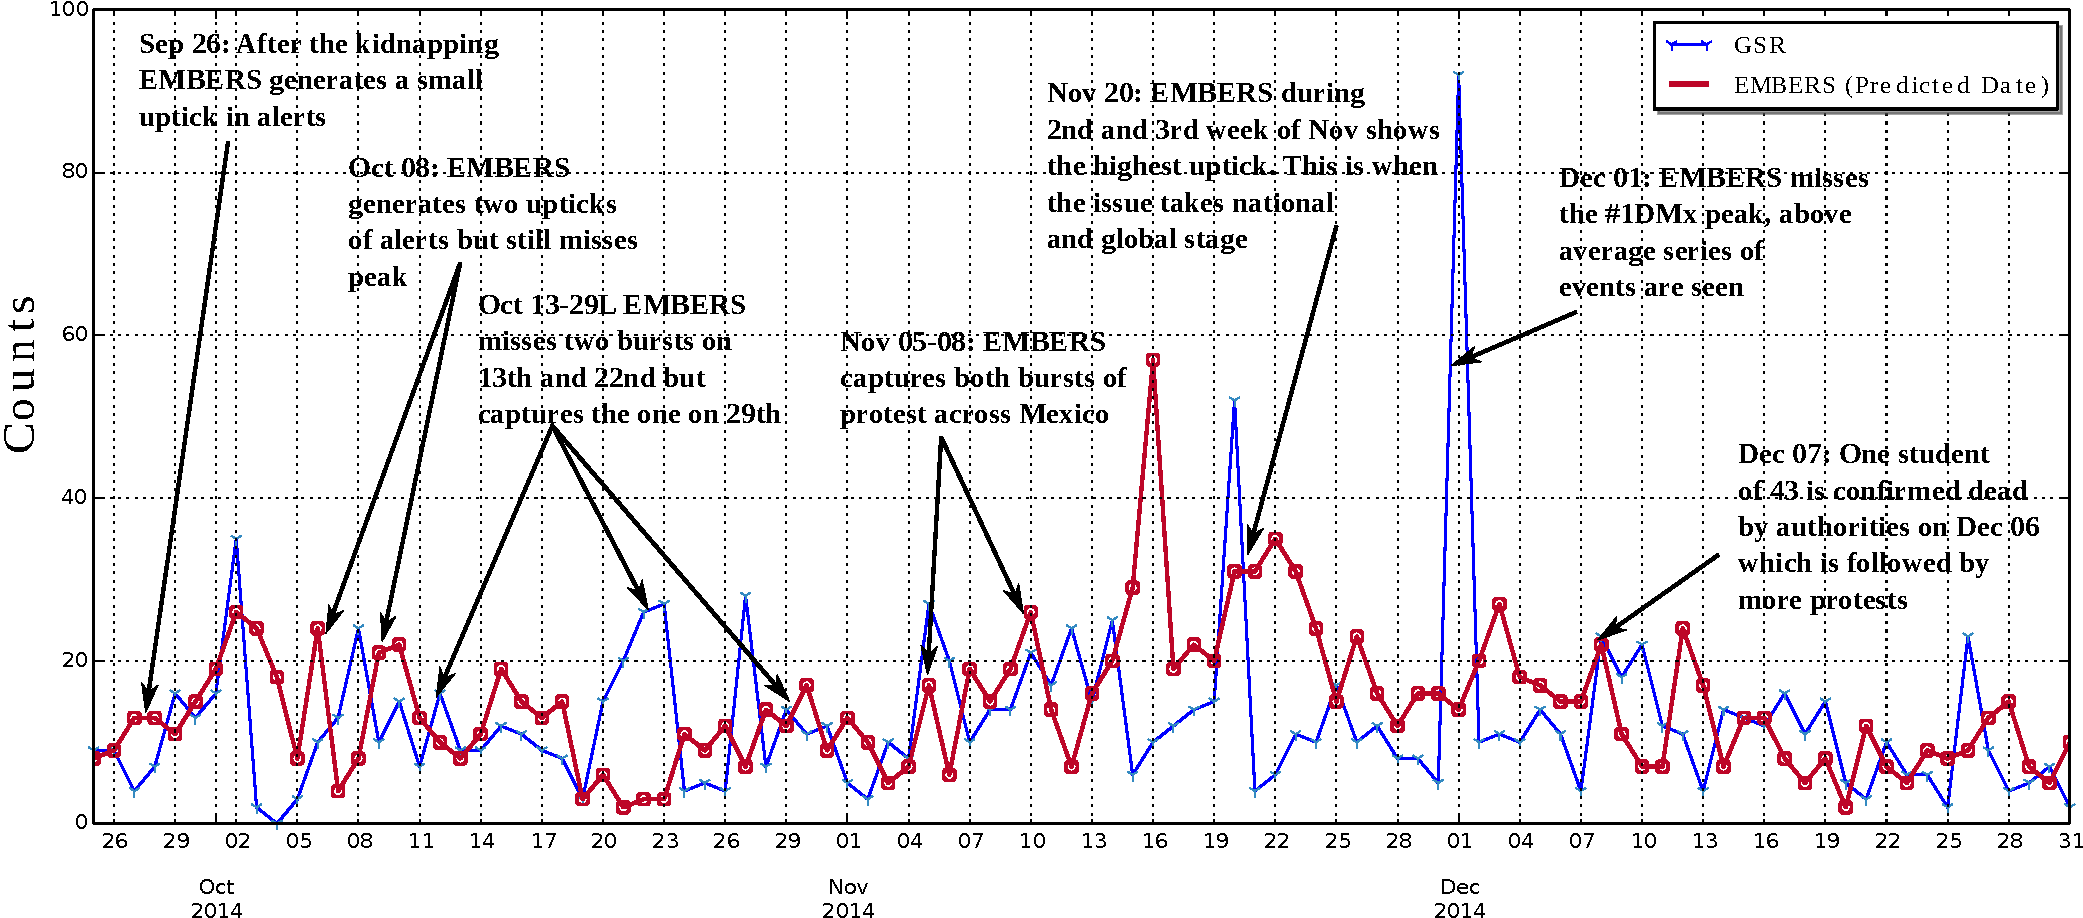
\includegraphics[width=.8\columnwidth]{cu/mx_timeline}
\caption{Mexico Protest timeline.The plot indicates the comparison between counts of GSR events
and EMBERS alerts’ for unique states/admins per day.The  }
EMBERS series’ as can be seen is more pronounced during Nov-Dec’14,
\label{fig:mexicoTimeline}
\end{figure}

\textbf{Colombia Protests (December'14 -March'15)}:
EMBERS successfully forecast the uptick in the number of events during the
middle of December 2014 and also the increase in protest counts during February
2015 as shown in Figure.~\ref{fig:colombiaDec14}, though in the latter case EMBERS over predicted the counts. The uptick in
December 2014 was led by the opposition leader Alvaro Uribe against impunity.
Whereas the increase in  protest counts in February 2015
was due to trucker’s strike against increase in fuel price.

\begin{figure}[H]
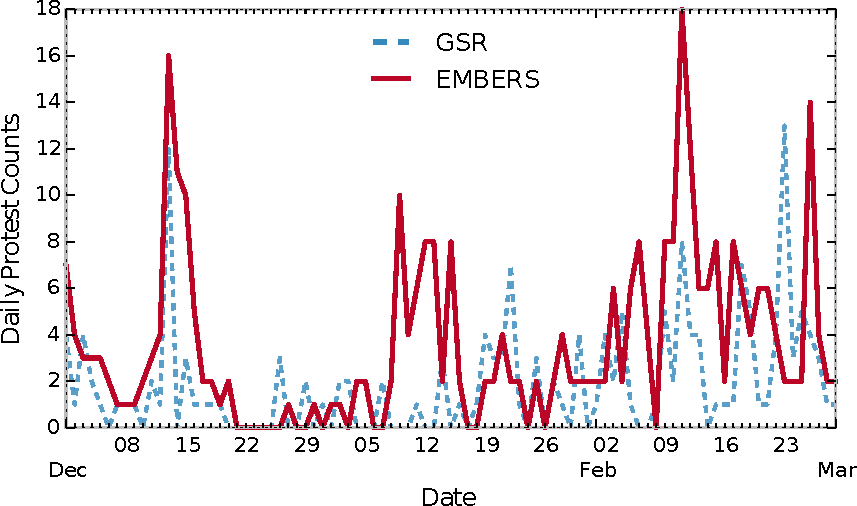
\includegraphics[width=.8\columnwidth]{cu/colombiaDec15}
\caption{Colombia Protests}
\label{fig:colombiaDec14}
\end{figure}

\textbf{Paraguay Protests (February 2015)}:
EMBERS forecast the uptick in number of protest events in Paraguay during mid
February 2015 as shown in Figure.~\ref{fig:paraguay15}. The events were mainly due to the lack of opportunity and basic
needs and against the introduction of new public-private partnership law.

\begin{figure}[H]
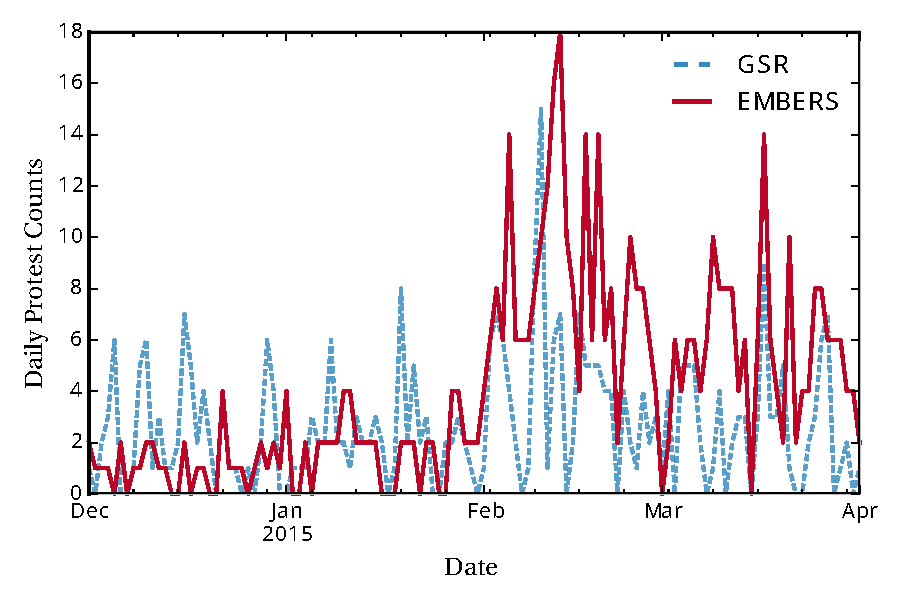
\includegraphics[width=.8\columnwidth]{cu/paraguayFeb15}
\caption{Paraguay Protests}
\label{fig:paraguay15}
\end{figure}


\subsection{Events missed by EMBERS}:
The following section details out certain events that EMBERS failed to
capture properly.

\textbf{Brazil Protests (March 2015)}: EMBERS predicted the accurate
increase in the rate of events but does not capture the true counts. The
protests were mainly targeted against president Dilma Rousseff due to
increasing corruption. 

During this period there was a significant architectural change in the
EMBERS processing pipeline. EMBERS had moved to Heideltime temporal
tagger from the previously used TIMEN temporal tagger due to
Heideltime`s support for more languages and active development cycle as
opposed to TIMEN. Heideltime had no support for portuguese (the main
language used in Brazil) and EMBERS team had extended Heideltime to
portuguese by translating the resources for spanish to portuguese. It
turned out that simple translation of rules from spanish to portuguese
were not sufficient and this affected the recall of one of our main
models for Brazil - Planned Protest - as it depended on the quality and recall of
date extraction from text.

\begin{figure}[H]
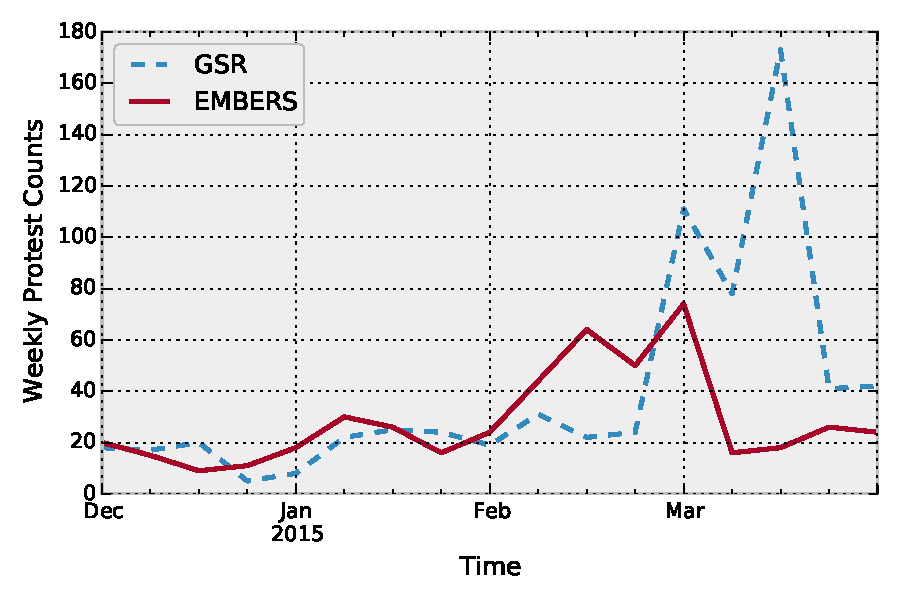
\includegraphics[width=.8\columnwidth]{cu/brazilMarch15}
\caption{Brazil 2015 Protests}
\label{fig:brazilSpring}
\end{figure}


\textbf{Mexico December 1, 2014 Protests}:
EMBERS missed the huge single day spike on December 1st when
people turned out in huge numbers in different parts of Mexico demanding
Pena Nieto`s ouster.
EMBERS predicted nationwide events for December 1st but failed to
capture the its spread. December 1st was picked by the protestors due to
its historical significance - it was the day when Pena Nieto was sworn
in as President in 2012 amidst much controversy and opposition from
general public. Also another reason was EMBERS inability in
extracting dates in twitter lingo  like "\#1Dmx".



